\part{一元积分}

\section{定积分}
\subsection{性质}
利用梯形逼近,定积分的定义如下
\begin{definition}
    设函数$f(x)$在闭区间$[a,b]$上有定义,如果存在$[a,b]$上的阶梯函数数列$\alpha_n(x),\beta_n(x)$使得
    \begin{enumerate}[(1)]
        \item 当$x\in[a,b]$且$n\geq 1$时,恒有$\alpha_n(x)\leq f(x)\leq \beta_n(x)$
        \item $\lim_{n\to\infty} \int_a^b \alpha_n(x)\dd{x} = \lim_{n\to\infty}\int_a^b \beta_n(x)\dd{x} = I$
    \end{enumerate}
    那么函数$f(x)$在$[a,b]$上的定积分为$\int_a^b f(x)\dd{x} = I$
\end{definition}

对于计算定积分,通常通过寻找原函数,再利用Newton-Leibniz公式计算。
\begin{theorem}
    (Newton-Leibniz公式)
    \label{th:Newton-Leibniz公式}
    如果函数$F(x)$是连续函数$f(x)$再区间$[a,b]$上的一个原函数,则
    \[ \int_a^bf(x)\dd{x} = F(b)-F(a) \]
\end{theorem}

可积函数的性质如下
\begin{theorem}
    函数$f(x)$在$[a,b]$上可积$\iff$对$\forall \epsilon > 0$,都$\exists [a,b]$上的阶梯函数
    $\alpha_n(x)$和$\beta_n(x)$使得
    \begin{enumerate}[(1)]
        \item 当$x\in[a,b]$时,恒有$\alpha_n(x)\leq f(x)\leq \beta_n(x)$
        \item $\int_a^b [\beta_n(x)-\alpha_n(x)] \dd{x} < \epsilon$
    \end{enumerate}
    推论:可积函数一定是有界函数
\end{theorem}

\begin{theorem}
    \marginnote{
        有界函数不一定可积,例如
        \[
            f(x) = \begin{cases}
                1, & x\text{ 为有理数} \\
                0, & x\text{ 为无理数}
            \end{cases}
        \]
        $f(x)$有界,但有无穷个间断点,故$f(x)$在任意的闭区间上不可积。
    }
    \begin{enumerate}
        \item 闭区间上的连续函数一定是可积函数。
        \item 闭区间上有界且最多只有\textcolor{red}{有限个}或\textcolor{red}{可数个}间断点的函数一定是可积函数。
        \item 闭区间上的单调有界函数一定是可积函数。
    \end{enumerate}
\end{theorem}

\begin{theorem}
    (积分线性性)
    设$f(x),g(x)$是$[a,b]$上的可积函数,$\lambda,\mu$是任意常数,
    则$f(x),g(x)$的线性组合$\lambda f(x)+\mu g(x)$是$[a,b]$上的可积函数,并且有
    \[
        \int_a^b \lambda f(x)+\mu g(x)\dd{x}
        =
        \lambda\int_a^b f(x)\dd{x} + \mu\int_a^b g(x)\dd{x}
    \]
\end{theorem}

\begin{theorem}
    (区间可加性)
    设函数$f(x)$是$[a,b]$上的可积函数,若$c\in(a,b)$,则
    \[ \int_a^b f(x)\dd{x} = \int_a^c f(x)\dd{x} + \int_c^b f(x)\dd{x} \]
\end{theorem}

\begin{theorem}
    (积分单调性)
    设$f(x),g(x)$是$[a,b]$上的可积函数,若$f(x)\leq g(x), \forall x \in (a,b)$则有
    \[ \int_a^b f(x)\dd{x} \leq \int_a^b g(x)\dd{x} \]

    推论:
    \begin{enumerate}[(1)]
        \item \[
                  \int_a^b f(x)\dd{x}
                  \begin{cases}
                      \geq 0 & f(x)\geq 0 \\
                      > 0    & f(x) > 0
                  \end{cases}
              \]
        \item 若$f(x),g(x)$不恒等,且$f(x)\leq g(x),\forall x \in (a,b)$,则有
              \[ \int_a^b f(x)\dd{x} < \int_a^b g(x)\dd{x} \]
        \item 若$m \leq f(x) \leq M$则有
              \[ m(b-a) \leq \int_a^b f(x)\dd{x} \leq M(b-a) \]
        \item 若$f(x)$非负,则对于子区间$[\alpha,\beta]$有
              \[ \int_\alpha^\beta f(x)\dd{x} < \int_a^bf(x)\dd{x} \]
    \end{enumerate}
\end{theorem}

\begin{theorem}
    (绝对可积性)
    \label{th:绝对可积性}
    设$f(x)$是$[a,b]$上的可积函数,则$\abs{f(x)}$在$[a,b]$上的可积函数,并且有
    \[ \abs{\int_a^b f(x)\dd{x}} \leq \int_a^b \abs{f(x)} \dd{x} \]
\end{theorem}

\begin{theorem}
    设$f(x)$在$[a,b]$上的连续函数,则存在$\xi\in(a,b)$,使得
    \[ \int_a^b f(x)\dd{x} = f(\xi)(b-a) \]
\end{theorem}

\begin{theorem}
    (积分中值定理)
    \label{th:积分中值定理}
    设$f(x)$在$[a,b]$上的连续函数,$g(x)$是$[a,b]$上的\textcolor{red}{不变号}可积函数,
    则$\exists \xi\in[a,b]$,使得
    \[ \int_a^b f(x)g(x)\dd{x} = f(\xi)\int_a^b g(x)\dd{x} \]
\end{theorem}

\subsubsection{奇偶函数、周期函数、含对称性函数、含有三角函数的定积分性质}
\paragraph{奇偶函数}
当定积分上下限对称,即积分区间为$[-a,a],a>0$时,奇偶函数$f(x)$的积分如下
\[
    \int_{-a}^a f(x)\dd{x} =
    \begin{cases}
        0,                   & f(x)\text{ 为奇函数} \\
        2\int_0^af(x)\dd{x}, & f(x)\text{ 为偶函数}
    \end{cases}
\]

\paragraph{周期函数}
当$f(x)$是以整数$T$为周期的连续函数,则对于任意的实数$a$,都有
\[\int_a^{a+T}f(x)\dd{x} = \int_0^T f(x)\dd{x} \]

\paragraph{含对称性函数}
若函数$f(x)$在$[a,b]$上可积,且$f(x)$关于$x=\dfrac{a+b}{2}$对称,那么可以令$t=x-\dfrac{a+b}{2}$
再根据偶函数的性质进行积分

当$f(x)$在$[a,b]$上可积时,且$f(x)$有某种轮换性质时,
可以通过$f(x)+f(a+b-x)$来简化定积分$\displaystyle\int_a^bf(x)\dd{x}$的计算。
其本质是在区间$[a,b]$上从左加到右,和从右加到左是一样的。
\begin{example}
    设$n$是正整数,计算$\displaystyle\int_0^{\frac{\pi}{2}}\frac{\sin^n x}{\sin^n x + \cos^n x}\dd{x}$
\end{example}
\begin{solution}
    令$t=\frac{\pi}{2}-x$,则有
    \begin{align*}
        \int_0^{\frac{\pi}{2}}\frac{\sin^n x}{\sin^n x + \cos^n x}\dd{x}
         & = \int_{\frac{\pi}{2}}^0\frac{\sin^n \left(\frac{\pi}{2}-t\right)}{\sin^n \left(\frac{\pi}{2}-t\right) + \cos^n \left(\frac{\pi}{2}-t\right)}\dd(\frac{\pi}{2}-t) \\
         & = \int_0^{\frac{\pi}{2}}\frac{\cos^n t}{\cos^n t + \sin^n t}\dd{t}
    \end{align*}
    根据$A = \frac{1}{2}(A+A)$可得
    \[
        \int_0^{\frac{\pi}{2}}\frac{\sin^n x}{\sin^n x + \cos^n x}\dd{x}
        =
        \frac{1}{2}\int_0^{\frac{\pi}{2}}\frac{\sin^n x + \cos^nx}{\sin^n x + \cos^n x}\dd{x}
        =
        \frac{1}{2}\int_0^{\frac{\pi}{2}} 1\dd{x}
        =
        \frac{\pi}{4}
    \]
\end{solution}

\begin{example}
    求定积分$\displaystyle\int_0^{\pi/2} \frac{1}{1+(\tan x)^{\sqrt{2}}}\dd{x}$
\end{example}
\begin{solution}
    \[
        \int_0^{\pi/2} \frac{1}{1+(\tan x)^{\sqrt{2}}}\dd{x}
        =
        \int_0^{\pi/2} \frac{(\cos x)^{\sqrt{2}}}{(\cos x)^{\sqrt{2}}+(\sin x)^{\sqrt{2}}}\dd{x}
    \]
    令$x=\frac{\pi}{2}-x$,则有
    \[
        \int_0^{\pi/2} \frac{(\cos x)^{\sqrt{2}}}{(\cos x)^{\sqrt{2}}+(\sin x)^{\sqrt{2}}}\dd{x}
        =
        \int_0^{\pi/2} \frac{(\sin x)^{\sqrt{2}}}{(\sin x)^{\sqrt{2}}+(\cos x)^{\sqrt{2}}}\dd{x}
    \]
    两式相加,则有
    \[
        \int_0^{\pi/2} \frac{1}{1+(\tan x)^{\sqrt{2}}}\dd{x}
        =
        \frac{1}{2} \int_0^{\pi/2} \frac{(\sin x)^{\sqrt{2}} + (\cos x)^{\sqrt{2}}}{(\sin x)^{\sqrt{2}}+(\cos x)^{\sqrt{2}}}\dd{x}
        =
        \frac{\pi}{4}
    \]
\end{solution}

\paragraph{含有三角函数}
设函数$f(x)$在$[0,1]$上连续,则有
\begin{enumerate}[(1)]
    \item $\displaystyle \int_0^{\pi/2}f(\sin x)\dd{x} = \int_0^{\pi/2}f(\cos x)\dd{x}$;
    \item $\displaystyle \int_0^{\pi}f(\sin x)\dd{x} = 2\int_0^{\pi/2}f(\sin x)\dd{x}$;
    \item $\displaystyle \int_0^{\pi}xf(\sin x)\dd{x} = \frac{\pi}{2}\int_0^{\pi}f(\sin x)\dd{x}$;
\end{enumerate}

\subsection{等式和不等式的证明}
含有积分的等式和不等式的证明,常用到以下几个知识点
\begin{enumerate}
    \item 积分中值定理(\ref{th:积分中值定理}),微分中值定理(\ref{th:罗尔定理}、\ref{th:拉格朗日中值定理}、\ref{th:柯西中值定理}),介值定理(\ref{th:介值定理})
    \item 泰勒公式(\ref{th:泰勒公式})
    \item 柯西不等式(\ref{eq:柯西不等式})、闵可夫斯基不等式(\ref{eq:闵可夫斯基不等式})
    \item 有绝对值时,绝对可积性(\ref{th:绝对可积性})、三角不等式(\ref{eq:三角不等式})、分段积分
    \item 将积分当作一个函数,研究其单调性和极值(最值)
    \item 被积函数的一些性质(单调性、周期性等)
\end{enumerate}
\begin{example}
    设函数$f(x)$在$[0,1]$上二阶可导,且$f(0)=f'(0)=f'(1)=0, f(1)=1$,
    证明:$\exists\xi\in(0,1)$,使得$\abs{f''(\xi)}\geq 4$
\end{example}
\begin{proof}
    注意到
    \begin{align*}
        f(b) - f(a) & = \int_a^b f'(x)\dd{x}                                                                \\
                    & = \int_a^b f'(x)\dd(x-t)                                                              \\
                    & = (b-t)f'(b)-(a-t)f'(a) - \int_a^b (x-t)f''(x)\dd{x} \qquad (\forall t\in \mathbf{R})
    \end{align*}
    当$f'(b)=f'(a)=0$时有
    \[ f(b) - f(a) = -\int_a^b (x-t)f''(x)\dd{x} \]
    由题意知$b=1,a=0$,由绝对可积性和积分中值定理可得
    \[
        1
        =
        \abs{\int_0^1 (x-t)f''(x)\dd{x}}
        \leq
        \int_0^1 \abs{x-t}\abs{f''(x)}\dd{x}
        = \abs{f''(\xi)}\int_0^1\abs{x-t}\dd{x}
    \]
    令$t=\frac{1}{2}$则有
    \[ 1 \leq \abs{f''(\xi)} \int_0^1\abs{x-\frac{1}{2}}\dd{x} = 4\abs{f''(\xi)} \qquad \xi\in(0,1)\]
    所以\[ \abs{f''(\xi)} \geq 4 \qquad \xi\in(0,1) \]
\end{proof}

\begin{example}
    设函数$f(x)$在$[a,b]$上二阶可导,且$f'(a)=f'(b)=0$,则$\exists\xi\in(a,b)$,使得
    \[ \abs{f''(\xi)} \geq \frac{4}{(b-a)^2}\abs{f(b)-f(a)} \]
\end{example}
\begin{proof}
    因为$f'(a)=f'(b)=0$,则有
    \[ f(b)-f(a) = -\int_a^b(x-t)f''(x)\dd{x} \qquad \forall t \in \mathbf{R}\]
    根据绝对可积性和积分中值定理得
    \[
        \abs{f(b)-f(a)}  = \abs{\int_a^b(x-t)f''(x)\dd{x}} \leq \int_a^b\abs{x-t}\abs{f''(x)}\dd{x} = \abs{f''(\xi)}\int_a^b\abs{x-t}\dd{x}
    \]
    其中$\xi\in(a,b)$,不妨令$t=\dfrac{a+b}{2}$,则有
    \begin{align*}
        \int_a^b\abs{x-t}\dd{x}
         & = \int_a^b \abs{x-\frac{a+b}{2}}\dd{x}                                                          \\
         & = \int_a^{\frac{a+b}{2}}(\frac{a+b}{2}-x)\dd{x} + \int_{\frac{a+b}{2}}^b(x-\frac{a+b}{2})\dd{x} \\
         & = \frac{(b-a)^2}{4}
    \end{align*}
    带入之前的不等式,可得
    \[ \abs{f''(\xi)} \geq \frac{4}{(b-a)^2}\abs{f(b)-f(a)} \]
\end{proof}

\begin{example}
    设$f(x),g(x)$在$[a,b]$上连续,证明至少存在一个$\xi\in(a,b)$,使得
    \[ f(\xi)\int_\xi^b g(x)\dd{x} = g(\xi)\int_a^\xi f(x)\dd{x} \]
\end{example}
\begin{proof}
    由于
    \begin{align*}
          & g(x)\int_a^x f(t)\dd{t} - f(x)\int_x^b g(t)\dd{t}   \\
        = & g(x)\int_a^x f(t)\dd{t} + f(x)\int_b^x g(t)\dd{t}   \\
        = & \left[\int_a^xg(t)\dd{t} \int_b^xf(t)\dd{t}\right]'
    \end{align*}
    故令
    \[ F(x) = \int_a^xg(t)\dd{t} \int_b^xf(t)\dd{t} \]
    由于$F(a)=F(b)=0$,由罗尔定理可得,存在$\xi\in(a,b)$
    \[ F'(\xi) = g(\xi)\int_a^\xi f(t)\dd{t} - f(\xi)\int_\xi^b g(t)\dd{t} = 0 \]
    即
    \[ f(\xi)\int_\xi^b g(x)\dd{x} = g(\xi)\int_a^\xi f(x)\dd{x} \]
\end{proof}

\begin{example}
    设$f(x),g(x)$在$[a,b]$上连续,且$g(x)\neq 0,\forall x\in(a,b)$,证明:
    \[ \exists \xi\in(a,b) , \frac{\int_a^bf(x)\dd{x}}{\int_a^bg(x)\dd{x}} = \frac{f(\xi)}{g(\xi)} \]
\end{example}
\begin{proof}
    由于
    \[
        g(x)\int_a^bf(t)\dd{t} - f(x)\int_a^bg(t)\dd{t}
        =
        \left[ \int_a^xg(t)\dd{t} \int_a^bf(t)\dd{t} - \int_a^xf(t)\dd{t} \int_a^bg(t)\dd{t} \right]'
    \]
    令
    \[ F(x) = \int_a^xg(t)\dd{t} \int_a^bf(t)\dd{t} - \int_a^xf(t)\dd{t} \int_a^bg(t)\dd{t} \]
    由于$F(a)=F(b)=0$,由罗尔定理知,$\exists\xi\in(a,b)$使得$F'(\xi)=0$,即
    \[ g(x)\int_a^bf(t)\dd{t} - f(x)\int_a^bg(t)\dd{t} = 0 \]
    所以有
    \[ \frac{\int_a^bf(x)\dd{x}}{\int_a^bg(x)\dd{x}} = \frac{f(\xi)}{g(\xi)} \]
\end{proof}

\begin{example}
    设函数$f(x)$在$[0,\pi]$上连续且
    \[ \int_0^\pi f(x)\cos x\dd{x} = \int_0^\pi f(x)\sin x\dd{x} = 0 \]
    求证:存在$0<x_1<x_2<\pi$,使得$f(x_1)=f(x_2)=0$
\end{example}
\begin{proof}
    因为在$(0,\pi)$上$\sin x > 0$,又$\int_0^\pi f(x)\sin x\dd{x} = 0$,
    所以$f(x)$在$(0,\pi)$上是变号函数,根据零点定理可知$f(x)$至少在$(0,\pi)$有一零点$x_0$,
    不妨假设$f(x)$只有一个零点$x_0$,则根据$f(x)$的连续性,

    当$f(x)>0,x\in(0,x_0)$和$f(x)<0,x\in(x_0,\pi)$时
    有
    \[ \sin(x-x_0)f(x) < 0 \]
    \[ \int_0^\pi \sin(x-x_0)f(x)\dd{x} < 0 \]

    当$f(x)<0,x\in(0,x_0)$和$f(x)>0,x\in(x_0,\pi)$时
    \[ \sin(x-x_0)f(x) > 0 \]
    \[ \int_0^\pi \sin(x-x_0)f(x)\dd{x} > 0 \]
    所以当$f(x)$只有一个零点$x_0$时
    \[ \int_0^\pi \sin(x-x_0)f(x)\dd{x} \neq 0 \]
    另一方面
    \[
        \int_0^\pi \sin(x-x_0)f(x)\dd{x}
        =
        \cos x_0\int_0^\pi \sin xf(x)\dd{x} - \sin x_0\int_0^\pi \cos xf(x)\dd{x}
        =
        0
    \]
    与假设所得不等式矛盾。故$f(x)$在$(0,\pi)$至少又两个零点。
\end{proof}
\begin{example}
    设函数$f(x),g(x)$是$[a,b]$上的连续增函数$(a>0)$,证明
    \[ \int_a^bf(x)\dd{x} \cdot \int_a^bg(x)\dd{x} \leq (b-a)\int_a^bf(x)g(x)\dd{x} \]
\end{example}
\begin{proof}
    通过函数单调性来证明:
    不妨设
    \[ F(x) = \int_a^xf(t)\dd{t} \cdot \int_a^xg(t)\dd{t} - (x-a)\int_a^xf(t)g(t)\dd{t} \]
    则
    \begin{align*}
        F'(x) & = f(x)\int_a^xg(t)\dd{t} + g(x)\int_a^xf(t)\dd{t} - \int_a^xf(t)g(t)\dd{t} - (x-a)f(x)g(x)          \\
              & =\int_a^xf(x)g(t)\dd{t} + \int_a^xf(t)g(x)\dd{t} - \int_a^xf(t)g(t)\dd{t} - \int_a^x f(x)g(x)\dd{t} \\
              & =\int_a^x[f(x)g(t) + f(t)g(x) - f(t)g(t) -  f(x)g(x)]\dd{t}                                         \\
              & =-\int_a^x[f(x)- f(t)][g(x) - g(t)]\dd{t} < 0
    \end{align*}
    所以$F(b)\leq F(a)=0$
\end{proof}

\begin{example}
    设$f(x)$在$[a,b]$上不恒为$0$,且其导数$f'(x)$连续,并且有$f(a)=f(b)=0$,证明存在$\xi\in[a,b]$使得
    \[ \abs{f'(\xi)} \geq \frac{4}{(b-a)^2} \int_a^b\abs{f(x)}\dd{x} \]
\end{example}
\begin{proof}
    通过微分中值定理求证\marginnote{由于命题得不等号和绝对可积性得不等号相反,故不用绝对可积性。}
    因为$f'(x)$在闭区间连续,故令$f'(\xi) = f'_{\max}(x)$

    根据拉格朗日中值定理有
    \[ \abs{f(x)} = \abs{f(x)-f(a)} = \abs{f'(\xi_1)}\abs{x-a} \leq \abs{f'(\xi)}(x-a) \]
    \[ \abs{f(x)} = \abs{f(x)-f(b)} = \abs{f'(\xi_2)}\abs{x-b} \leq \abs{f'(\xi)}(b-x) \]
    所以
    \begin{align*}
        \int_a^b\abs{f(x)}\dd{x} & = \int_a^{\frac{a+b}{2}} \abs{f(x)}\dd{x} + \int_{\frac{a+b}{2}}^b \abs{f(x)}\dd{x}                      \\
                                 & \leq \abs{f'(\xi)}\left[ \int_a^{\frac{a+b}{2}} (x-a)\dd{x} + \int_{\frac{a+b}{2}}^b (b-x)\dd{x} \right] \\
                                 & = \frac{(b-a)^2}{4}\abs{f'(\xi)}
    \end{align*}
    由此可知原命题成立。
\end{proof}

\begin{example}
    设$f(x)$在$[a,b]$上单调增,且$f''(x)>0$,证明
    \[ (b-a)f(a)<\int_a^bf(x)\dd{x} < (b-a)\cdot\frac{f(a)+f(b)}{2} \]
\end{example}
\begin{marginfigure}
    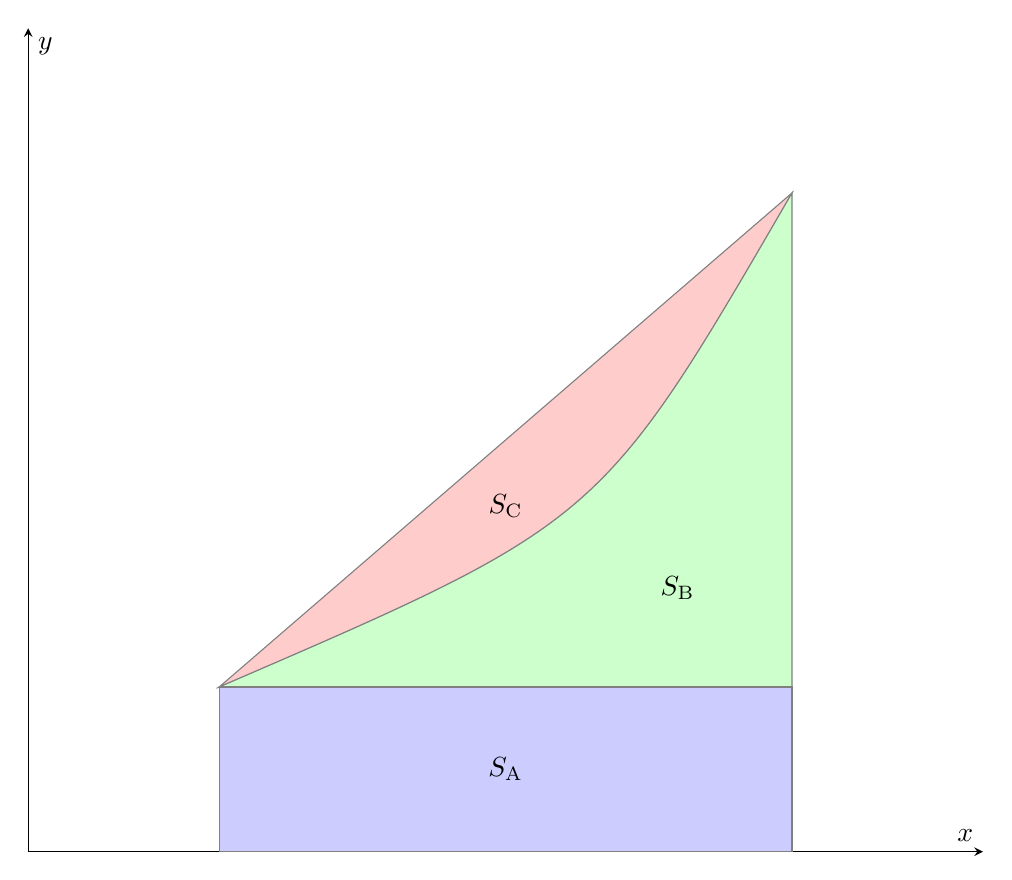
\begin{tikzpicture}
        \begin{axis}[
                ticks=none,
                axis x line=middle,
                axis y line=middle,
                xmin=0, xmax=2.5,
                ymin=0, ymax=2.5,
                xlabel=$x$,
                ylabel=$y$,
                scale only axis,
                width=\textwidth
            ]
            \coordinate (A) at (0.5, 0);
            \coordinate (B) at (0.5, 0.5);
            \coordinate (C) at (2, 2);
            \coordinate (D) at (2, 0.5);
            \coordinate (E) at (2, 0);
            \draw [Gray,fill=red!20!white] (B) .. controls (1.5, 1) .. (C) --cycle;
            \draw [Gray,fill=green!20!white] (B) .. controls (1.5, 1) .. (C) -- (D) -- cycle;
            \draw [Gray,fill=blue!20!white] (A) -- (B) -- (D) -- (E) --cycle;
            \node [Black] at (1.25, 0.25) {$S_\mathrm{A}$};
            \node [Black] at (1.7, 0.8) {$S_\mathrm{B}$};
            \node [Black] at (1.25, 1.05) {$S_\mathrm{C}$};
        \end{axis}
    \end{tikzpicture}
    \caption{$S_\mathrm{A} < S_\mathrm{A}+S_\mathrm{B} < S_\text{A}+S_\mathrm{B}+S_\mathrm{C} $}
\end{marginfigure}
\begin{proof}
    因为$f(x)$单调增,所以$f'(x)\geq 0$,又因为$f''(x)>0$,所以$f'(x)$单调增,故$f'(x)$不恒为零,所以$f(x)$不恒为$f(a)$。
    \[ \int_a^bf(x)\dd{x} > \int_a^b f(a)\dd{x} =(b-a)f(a) \]
    所以不等式左侧成立,下证不等式右侧

    因为$f''(x)>0$,所以$f(x)$为凹函数,故有
    \[ f(x) < \frac{f(b)-f(a)}{b-a}(x-a) + f(a) \]
    因此
    \[
        \int_a^bf(x)\dd{x}
        <
        \int_a^b \frac{f(b)-f(a)}{b-a}(x-a) + f(a) \dd{x}
        =
        (b-a)\cdot\frac{f(a)+f(b)}{2}
    \]
\end{proof}

\begin{example}
    设$\displaystyle f(x) = \ln x - x\int_1^\mathrm{e}\frac{f(x)}{x}\dd{x}$,
    求$f(x)$
\end{example}
\begin{solution}
    \[
        \frac{f(x)}{x} = \frac{\ln x}{x} - \int_1^\mathrm{e}\frac{f(x)}{x}\dd{x}
        =
        \frac{\ln x}{x} - A
    \]
    两边同时在$[1,\mathrm{e}]$上积分,
    \[
        A
        =
        \int_1^\mathrm{e}\frac{f(x)}{x}\dd{x}
        =
        \int_1^\mathrm{e}\frac{\ln x}{x}\dd{x} - \int_1^\mathrm{e} A\dd{x}
        =
        \frac{1}{2} - A(\mathrm{e}-1)
    \]
    所以$A = \dfrac{1}{2\mathrm{e}}$,带入原式得
    \[ f(x) = \ln x - \frac{x}{2\mathrm{e}} \]
\end{solution}

\begin{example}
    设$\displaystyle F(x) = \int_x^{x+2\pi} \mathrm{e}^{\sin t}\sin t\dd{t}$,
    证明:$F(x)$恒为正常数。
\end{example}

\begin{proof}
    设$f(x)= \mathrm{e}^{\sin x}\sin x$,显然$f(x+2\pi) = f(x)$,则$f(x)$是以$2\pi$为周期的连续函数。
    故
    \begin{align*}
        F(x) & = \int_0^{2\pi} \mathrm{e}^{\sin t}\sin t\dd{t}                                                  \\
             & = \int_0^{\pi}\mathrm{e}^{\sin t}\sin t\dd{t} + \int_{\pi}^{2\pi}\mathrm{e}^{\sin t}\sin t\dd{t} \\
             & = \int_0^{\pi}\mathrm{e}^{\sin t}\sin t\dd{t} - \int_0^{\pi}\mathrm{e}^{-\sin t}\sin t\dd{t}     \\
             & = \int_0^{\pi}\left(\mathrm{e}^{\sin t} - \mathrm{e}^{-\sin t}\right)\sin t\dd{t}                \\
    \end{align*}
    因为在$[0,\pi]$上$\sin x > 0$,所以$\left(\mathrm{e}^{\sin x} - \mathrm{e}^{-\sin x}\right)\sin x >0$,
    故$F(x)$恒为正常数。
\end{proof}

\begin{example}
    设$f(x)$在$[a,b]$上二阶连续可微,且$\displaystyle f\left(\frac{a+b}{2}\right)=0$,证明
    \[ \abs{\int_a^bf(x)\dd{x}} \leq \frac{M}{24}(b-a)^3  \]
    其中$M=\max_{a\leq x \leq b}\abs{f''(x)}$
\end{example}
\begin{proof}
    由题意根据泰勒公式得,其中$t=\dfrac{a+b}{2},\xi $在$t$的去心领域内
    \[
        f(x)  = f(t) + f'(t)(x-t)+ \frac{1}{2}f''(\xi)(x-t)^2
        = f'(t)(x-t) + \frac{1}{2}f''(\xi)(x-t)^2
    \]
    左右绝对积分得
    \begin{align*}
        \abs{\int_a^bf(x)\dd{x}}
         & = \abs{\int_a^bf'(t)(x-t) + \frac{1}{2}f''(\xi)(x-t)^2\dd{x}}                          \\
         & \leq \abs{\int_a^b f'(t)(x-t)\dd{x}} + \abs{\int_a^b \frac{1}{2}f''(\xi)(x-t)^2\dd{x}} \\
         & = 0 + \frac{1}{2}\abs{\int_a^b f''(\xi)(x-t)^2\dd{x}}                                  \\
         & \leq \frac{M}{2}\int_a^b (x-t)^2\dd{x}                                                 \\
         & =\frac{M}{6}[(b-t)^3 - (a-t)^3]                                                        \\
         & =\frac{M}{24}(b-a)^3
    \end{align*}
\end{proof}
解此题首先要将已知的条件往结论的形式上凑。这里有一个难点是,将一个定积分拆成两个定积分,任意其中一个定积分进行变量代换时,对另一个定积分无影响。
同时积分函数相同,且上下限能合并,那么无论积分微元是$t$还是$x$,都可以合并。对于上下限相同,函数合并,是同理的。
其本质是
\[
    \int_a^b f(x)\dd{x} + \int_b^c f(x)\dd{t}
    =
    \sum_{i=n_1}^{n_2-1} a_i + \sum_{i=n_2}^{n_3-1} a_i
    =
    \sum_{i=n_1}^{n_3} a_i = \int_a^c f(x)\dd{x}
\]
\[
    \int_a^b f(x)\dd{x} + \int_a^b g(t)\dd{t}
    =
    \sum a_i + \sum b_i = \sum (a_i + b_i)
    =
    \int_a^b f(x)+g(x)\dd{x}
\]
\begin{example}
    设$f(x)$在$[0,+\infty)$上连续,$0<a<b$,且$\displaystyle\int_A^{+\infty}\frac{f(x)}{x}\dd{x}$收敛,其中常数$A>0$,证明
    \[
        \int_0^{+\infty}\frac{f(ax)-f(bx)}{x}\dd{x} = f(0)\ln\frac{b}{a}
    \]
\end{example}
\begin{proof}
    因为
    \[ \int_A^{+\infty}\frac{f(x)}{x}\dd{x} = \int_{A/a}^{+\infty} \frac{f(ax)}{x}\dd{x} \]
    \[ \int_A^{+\infty}\frac{f(x)}{x}\dd{x} = \int_{A/b}^{+\infty} \frac{f(bx)}{x}\dd{x} \]
    那么有
    \begin{align*}
        \int_\varepsilon^{+\infty} \frac{f(ax)-f(bx)}{x}\dd{x}
         & = \int_\varepsilon^{+\infty} \frac{f(ax)}{x}\dd{x} - \int_\varepsilon^{+\infty}\frac{f(bx)}{x}\dd{x}     \\
         & = \int_{a\varepsilon}^{+\infty} \frac{f(t)}{t}\dd{t} - \int_{b\varepsilon}^{+\infty}\frac{f(t)}{t}\dd{t} \\
         & = \int_{a\varepsilon}^{b\varepsilon} \frac{f(x)}{x}\dd{x}                                                \\
         & = f(\xi)\int_{a\varepsilon}^{b\varepsilon} \dd{\ln x} \qquad \xi\in(a\varepsilon,b\varepsilon)           \\
         & = f(\xi)\ln\frac{b}{a} \qquad                                                                            \\
    \end{align*}
    那么当$\xi\to 0^+$时,则有$f(\xi)=f(0)$,所以
    \[
        \int_0^{+\infty}\frac{f(ax)-f(bx)}{x}\dd{x} = f(0)\ln\frac{b}{a}
    \]
\end{proof}

\begin{example}
    设函数$f'(x)$在$[a,b]$上连续,且$f(a)=0$,证明
    \[ \int_a^b f^2(x)\dd{x} \leq \frac{(b-a)^2}{2}\int_a^b[f'(x)]^2\dd{x} \]
\end{example}
\begin{proof}
    由命题的形式可以联想到柯西不等式\ref{eq:柯西不等式},所以我们尽量往柯西不等式凑。
    \[
        \left(\int_a^x f'(t)\dd{t}\right)^2
        \leq
        \left(\int_a^x [f'(t)]^2\dd{t}\right)\cdot\left(\int_a^x 1^2\dd{t}\right)
        =
        (x-a)\int_a^x [f'(t)]^2\dd{t}
    \]
    而
    \[ \left(\int_a^x f'(t)\dd{t}\right)^2 = \left(f(x)-f(a)\right)^2 = f^2(x) \]
    所以有
    \[ 0 \leq f^2(x) \leq (x-a)\int_a^x [f'(t)]^2\dd{t} \]
    左右同时积分可得
    \begin{align*}
        \int_a^b f^2(x)\dd{x}
         & \leq
        \int_a^b (x-a)\int_a^x [f'(t)]^2\dd{t}\dd{x}  \\
         & \leq
        \int_a^b (x-a)\int_a^b [f'(t)]^2\dd{t}\dd{x}  \\
         & =
        \int_a^b (x-a)\dd{x} \int_a^b [f'(t)]^2\dd{t} \\
         & =
        \frac{(b-a)^2}{2} \int_a^b [f'(x)]^2\dd{x}
    \end{align*}
\end{proof}
上述证明中的难点是对于$f^2(x)\geq 0$,则子区间的定积分(或变限积分)小于原区间的定积分,同时定积分是一个数,
可以从双重积分中提出,再变换积分微元,此做法的本质如下
\[ \sum \left(a_i\sum b_j\right) = a_1\sum b_j + a_2\sum b_j + \cdots a_n\sum b_j = \sum a_i\cdot\sum b_j = \sum a_i\cdot\sum b_i \]

利用单调性的解法如下
\begin{proof}
    设
    \[ F(x) = \int_a^xf^2(t)\dd{t} - \frac{(x-a)^2}{2}\int_a^x[f'(t)]^2\dd{t} \]
    那么$F(a)=0$,同时
    \begin{align*}
        F'(x)
         & = f^2(x) - (x-a)\int_a^x[f'(t)]^2\dd{t} - \frac{(x-a)^2}{2}[f'(x)]^2              \\
         & = f^2(x) - \int_a^x 1^2\dd{x}\int_a^x[f'(t)]^2\dd{t} - \frac{(x-a)^2}{2}[f'(x)]^2 \\
         & \leq f^2(x) - \left(\int_a^xf'(t)\dd{t}\right)^2 - \frac{(x-a)^2}{2}[f'(x)]^2     \\
         & =f^2(x) - (f(x)-f(a))^2 - \frac{(x-a)^2}{2}[f'(x)]^2                              \\
         & =- \frac{(x-a)^2}{2}[f'(x)]^2                                                     \\
         & \leq 0
    \end{align*}
    所以$F(x)$单调递减,则$F(b) \leq F(a) = 0$,即
    \[ \int_a^b f^2(x)\dd{x} \leq \frac{(b-a)^2}{2}\int_a^b[f'(x)]^2\dd{x} \]
\end{proof}

\subsection{面积、体积计算}
\subsubsection{\texorpdfstring{$x$}{x}型区域的面积}
由上下两条曲线$y_\text{上}=f(x),y_\text{下}=g(x)$以及左右两条直线$x=a,x=b$所围成的区域面积
\[ S = \int_a^b [f(x)-g(x)]\dd{x} \]

\subsubsection{\texorpdfstring{$y$}{x}型区域的面积}
与$x$型区域的面积类似,由左右两条曲线围成$x_\text{左}=\psi(y),x_\text{右}=\varphi(y)$以及上下两条直线$y=d,y=c$所围成的区域面积
\[ S = \int_c^d [\varphi(y)-\psi(y)]\dd{y} \]

\subsubsection{参数型区域的面积}
如果曲边梯形的上边界由参数方程$x=x(t),y=y(t)\ (\alpha<t<\beta)$所确定,则有
\[ S = \int_\alpha^\beta y(t)\dd{x}(t) \]

\subsubsection{极坐标型区域的面积}
若极坐标曲线$r=f(\theta)$是连续的,那么由$r=f(\theta)$和射线$\theta=\alpha,\theta=\beta$所围成的扇形面积为
\[ S = \frac{1}{2}\int_\alpha^\beta f^2(\theta)\dd{\theta} \]

\subsubsection{几何体体积的截面算法}
如果一个集合体在$x$轴的正投影区间为$[a,b]$,并且在每一点$x\in[a,b]$的横截面积为$S(x)$,
那么当$S(x)$在$[a,b]$上连续时,该集合体体积为
\[ V = \int_a^b S(x)\dd{x} \]

\subsubsection{旋转体体积的柱形算法}
如果选旋转体是由在区间$[a,b]$上的连续曲线$y=f(x)$绕$x$轴旋转一周所形成,那么其体积为
\[ V = \pi\int_a^bf^2(x)\dd{x} \]

当所求旋转体是由两条曲线$y_1=f(x),y_2=g(x)$所夹区域,绕$x$轴旋转一周形成,且$\abs{f(x)} > \abs{g(x)}$恒成立,那么体积为
\[ V = V_1 - V_2 = \pi\int_a^b f^2(x)-g^2(x)\dd{x} \]

\subsubsection{旋转体体积的管形算法}
如果旋转体由曲边梯形
\[ 0\leq y \leq f(x), a\leq x \leq b \]
绕$y$轴生成那么其体积微元为
\[ \Delta V = \pi(x+\Delta x)^2y - \pi x^2y = 2\pi xy\Delta x + \pi y\Delta x^2  \]
取线性主部积分,那么体积为
\[ V = 2\pi\int_a^bxf(x)\dd{x} \]

\subsubsection{显式曲线的弧长}
如果曲线$L$是由连续可微函数$y=f(x),x\in[a,b]$给出,则$L$是可求长曲线,
则弧长微元为
\[ \Delta s = \sqrt{\Delta x^2 + \Delta y^2} = \sqrt{1+\left(\frac{\Delta y}{\Delta x}\right)^2}\cdot \Delta x \]
因此弧长公式为
\[ s = \int_a^b \sqrt{1+[f'(x)]^2}\dd{x} \]

\subsubsection{参数曲线弧长}如果$L: x=x(t), y=y(t),t\in[a,b]$是一条不自交的连续可微曲线,则有
\[ s = \int_a^b\sqrt{x'^2+y'^2}\dd{t} \]

\subsubsection{极坐标曲线的弧长}
如果连续可微的曲线的极坐标方程为$r=r(\theta),\theta\in[\alpha,\beta]$则其参数方程为
\[ x = r(\theta)\cos\theta,y=r(\theta)\sin\theta,\theta\in[\alpha,\beta] \]
根据参数曲线的弧长公式可知
\[ s = \int_\alpha^\beta \sqrt{r^2+r'^2}\dd{\theta} \]

\section{不定积分}
定积分的计算可以寻找原函数后,再通过Newton-Leibniz公式\ref{th:Newton-Leibniz公式}计算,因此研究原函数就是不定积分的计算
\begin{definition}
    设函数$f(x)$是$[a,b]$上的连续函数,则面积函数
    \[ F(x) = \int_a^x f(t)\dd{t} \]
    是$[a,b]$上的可导函数,且$F'(x)=f(x)$
\end{definition}
\begin{definition}
    如果在区间$I$上,可导函数$F(x)$的导函数为$f(x)$,即当$x\in I$时,恒有
    \[ F'(x) = f(x) \]
    则称$F(x)$时$f(x)$在区间$I$上的一个原函数。
    注:连续函数的面积函数是其中一个原函数。
\end{definition}
\begin{definition}
    函数$f(x)$在区间$[a,b]$上的全体原函数成为$f(x)$再$[a,b]$上的不定积分,记作$\int f(x)\dd{x}$

    如果$F(x)$是函数$f(x)$再区间$[a,b]$上的一个原函数,则有
    \[\int f(x)\dd{x} = \left\{F(x)+C \,\middle|\, C\in\mathbf{R} \right\} \]
\end{definition}

在原函数的定义中可知,原函数一定可导,所以原函数一定连续,(原函数的导函数在区间\textcolor{red}{可以不连续}(看下题的注释),但在区间的每个都有定义,即导函数有值)。
\begin{example}
    证明:含第一类间断点、无穷型第二类间断点的函数$f(x)$在包含该间断点的区间内没有原函数$F(x)$
\end{example}
\begin{proof}
    假设$F(x)$为$f(x)$的原函数,那么有$F'(x)=f(x)$,设$x=x_0$为间断点,由题意可知$f(x_0)$有定义,
    在下面分类讨论
    \begin{enumerate}[(1)]
        \item 当$x=x_0$为第一类可去间断点时,即$\lim_{x\to x_0} f(x) \neq f(x_0)$,则有
              \begin{align*}
                  f(x_0) = F'(x_0) & = \lim_{x\to x_0}\frac{F(x)-F(x_0)}{x-x_0}     \\
                                   & =\lim_{x\to x_0}F'(x) \qquad \text{洛必达法则} \\
                                   & = \lim_{x\to x_0} f(x)
              \end{align*}
              矛盾,所以$F(x)$不存在。
        \item 当$x=x_0$为第一类跳跃间断点时,不妨令$\lim_{x\to x^-} f(x) \neq \lim_{x\to x^+}$
              \begin{align*}
                  f(x_0) = F'(x_0) & = \lim_{x\to x_0}\frac{F(x)-F(x_0)}{x-x_0}     \\
                                   & =\lim_{x\to x_0}F'(x) \qquad \text{洛必达法则} \\
                                   & = \lim_{x\to x_0} f(x)
              \end{align*}
              由于$f(x_0)$存在,但$\lim_{x\to x_0} f(x)$不存在,矛盾,所以$F(x)$不存在。
        \item 无穷型第二类间断点的函数与(2)同理可证。
    \end{enumerate}
    注:非无穷型的第二类间断点(非无穷振荡点)的函数,可以有原函数,因具体分析,如
    \[
        F(x)=
        \begin{cases}
            x^2\sin\frac{1}{x}, & x\neq 0, \\
            0,                  & x=0
        \end{cases}
    \]
    是
    \[
        f(x)=
        \begin{cases}
            2x\sin\frac{1}{x} - \cos\frac{1}{x}, & x\neq 0, \\
            0,                                   & x=0
        \end{cases}
    \]
    的原函数。
    而
    \[
        f(x)=
        \begin{cases}
            \sin\frac{1}{x}, & x\neq 0, \\
            0,               & x=0
        \end{cases}
    \]
    不存在原函数。
\end{proof}

\subsection{积分方法}
\subsubsection{换元积分法}
大多数的积分需要通过变量代换化简后计算,也称换元积分法
\begin{theorem}
    (第一类换元法)
    设函数$f(u)$存在原函数,$u=\varphi(x)$可导,则
    \[ \int f\circ\varphi(x)\cdot \varphi'(x)\dd{x} = \eval{\int f(u)\dd{u}}_{u=\varphi(x)} \]
    若函数$u=\varphi(x)$在区间$I=[a,b]$上连续可导,
    函数$f(u)$在区间$\varphi(I)=\left\{\varphi(x) \,\middle|\, x\in[a,b]\right\}$上连续,
    若$\alpha=\varphi(a),\beta=\varphi(b)$,则
    \[
        \int_a^b f\circ\varphi(x)\cdot\varphi'(x)\dd{x}
        =
        \int_{\varphi(a)}^{\varphi(b)} f(u)\dd{u}
        =
        \int_\alpha^\beta f(u)\dd{u}
    \]
\end{theorem}

\begin{example}
    求$\displaystyle\int \frac{1}{\sin^2 x + 2\cos^2 x}\dd{x}$
\end{example}
\begin{solution}
    \begin{align*}
        \int \frac{1}{\sin^2 x + 2\cos^2 x}\dd{x}
         & = \int \frac{1}{\tan^2 x + 2}\frac{\dd{x}}{\cos^2 x}            \\
         & = \int \frac{1}{\tan^2 x + (\sqrt{2})^2} \dd{\tan x}            \\
         & = \frac{1}{\sqrt{2}}\arctan\left(\frac{\tan x}{\sqrt{2}}\right)
    \end{align*}
\end{solution}


\begin{theorem}
    (第二类换元法)
    设$x=\varphi(t)$在区间$I$上连续可导且$\varphi'(t)\neq 0$,若$f(x)$在区间$\varphi(I)$上存在原函数,则
    \[ \int f(x)\dd{x} = \eval{\int f\circ\varphi(t)\cdot\varphi'(t)\dd{t}}_{t=\varphi^{-1}(x)} \]
\end{theorem}
\begin{situation}
    第二类换元法是第一类换元法的反向使用,也称“拆微分”。当被积函数中部分项比较复杂,或存在三角代换、双曲代换时,可使用此方法。
\end{situation}

\subsubsection{分部积分法}
由于$(uv)'=u'v+uv'$,所以有
\begin{theorem}
    (分部积分法)
    设$u=u(x),v=v(x)$是区间$[a,b]$上的连续可导函数,则
    \[ \int u\dd{v} = uv - \int v\dd{u} \qquad \int_a^b u\dd{v} = \eval{uv}_a^b - \int_a^bv\dd{u} \]
\end{theorem}
\begin{situation}
    分部积分法适用于含$\mathrm{e}^x,\ln x$和三角函数的积分,因为其多次求导具有周期的性质,或可以与某些项相消,故多次使用分部积分法后移项,即可求出积分。
    \begin{alignat*}{43}
         & \int P_n(x)\mathrm{e}^{kx}\dd{x}     & = &   & \frac{1}{k} & \int P_n(x)\dd{\mathrm{e}^kx)}      \\
         & \int P_n(x)\sin ax\dd{x}             & = & - & \frac{1}{a} & \int P_n(x)\dd{\cos ax}             \\
         & \int P_n(x)\cos ax\dd{x}             & = &   & \frac{1}{a} & \int P_n(x)\dd{\sin ax}             \\
         & \int \mathrm{e}^{kx}\sin(ax+b)\dd{x} & = & - & \frac{1}{a} & \int \mathrm{e}^{kx}\dd{\cos(ax+b)} \\
         & \int \mathrm{e}^{kx}\cos(ax+b)\dd{x} & = &   & \frac{1}{a} & \int \mathrm{e}^{kx}\dd{\sin(ax+b)} \\
         & \int P_n'(x)\ln x\dd{x}              & = &   &             & \int \ln x\dd{P_n(x)}               \\
         & \int P_n'(x)\arcsin x\dd{x}          & = &   &             & \int \arcsin x\dd{P_n(x)}           \\
         & \int P_n'(x)\arccos x\dd{x}          & = &   &             & \int \arccos x\dd{P_n(x)}
    \end{alignat*}

    其中$P_n(x)$为$n$次多项式,$k,a,b$为常数
\end{situation}
利用分部积分法,还可以建立一些不定积分的递推公式
\begin{example}
    求$I_n=\int \sin^n x\dd{x}$
\end{example}
\begin{solution}
    \begin{align*}
        I_n & = \int \sin^{n-1} x \dd(-\cos x)                                            \\
            & = -\cos x\sin^{n-1}x + \int \cos x\cdot(n-1)\sin^{n-2}x\cos x\dd{x}         \\
            & = -\cos x\sin^{n-1}x + (n-1)\int (1-\cos^2 x)\sin^{n-2}x\dd{x}              \\
            & = -\cos x\sin^{n-1}x + (n-1)\int \sin^{n-2}x\dd{x} - (n-1)\int\sin^nx\dd{x} \\
            & = -\cos x\sin^{n-1}x + (n-1)I_{n-2} - (n-1)I_n
    \end{align*}
    所以
    \[ I_n = -\frac{1}{n}\cos x\sin^{n-1}x + \frac{n-1}{n}I_{n-2} \]
\end{solution}

\subsubsection{三角乘积的积分}
在含三角乘积的积分中,常用到半角公式
\[ \cos^2x = \frac{1+\cos 2x}{2}, \qquad \sin^2 x = \frac{1-\cos 2x}{2} \]
与积化和差公式
\begin{align*}
    \sin\alpha\cos\beta & = \frac{1}{2}[\sin(\alpha+\beta)+\sin(\alpha-\beta)] \\
    \sin\alpha\sin\beta & = \frac{1}{2}[\cos(\alpha-\beta)-\cos(\alpha+\beta)] \\
    \cos\alpha\cos\beta & = \frac{1}{2}[\cos(\alpha+\beta)+\cos(\alpha-\beta)]
\end{align*}

\begin{example}
    求$\displaystyle \int\sin 3x\sin 2x\dd{x}$
\end{example}
\begin{solution}
    \[
        \int\sin 3x\sin 2x\dd{x}
        =
        \frac{1}{2}\int [\cos(3x-2x) - \cos(3x+2x)] \dd{x}
        =
        \frac{1}{2}\sin x - \frac{1}{10}\sin 5x + C
    \]
\end{solution}
\begin{example}
    求$\displaystyle \int(1+\cos 3x)^{3/2}\dd{x}$
\end{example}
\begin{solution}
    利用半角公式有
    \begin{align*}
        \int(1+\cos 3x)^{3/2}\dd{x} & = 2\sqrt{2}\int \cos[3](\frac{3x}{2})\dd{x}                                            \\
                                    & = \frac{4\sqrt{2}}{3}\int \left[1-\sin[2](\frac{3x}{2})\right]\dd{\sin(\frac{3x}{2})}  \\
                                    & = \frac{4\sqrt{2}}{3}\sin(\frac{3x}{2}) - \frac{4\sqrt{2}}{9}\sin[3](\frac{3x}{2}) + C \\
                                    & = \frac{4\sqrt{2}}{9}\left[3\sin(\frac{3x}{2})-\sin[3](\frac{3x}{2})\right] + C
    \end{align*}
\end{solution}

\subsubsection{万能公式求解三角函数积分}
若被积函数为含三角函数的分式时,且不好“凑微分”、化简时,可以利用三角函数的万能公式将其转化为有理分式的积分。
\begin{align}
    \label{eq:万能公式}
    \sin x & = \frac{2t}{1+t^2}    \\
    \cos x & = \frac{1-t^2}{1+t^2} \\
    \tan x & = \frac{2t}{1-t^2}
\end{align}
其中$t=\tan \frac{x}{2}$。

其本质是三角函数的降角升幂,同时提取$\sec^2\frac{x}{2}$,使得不定积分变为
\[ \int f(x)\dd{x} = 2\int \sec^2\frac{x}{2}\cdot g\left(\tan\frac{x}{2}\right) \dd{\frac{x}{2}} = 2\int g\left(\tan\frac{x}{2}\right)\dd{\tan\frac{x}{2}} \]

\begin{example}
    求$\displaystyle\int\frac{\dd{x}}{2+\sin x}$
\end{example}
\begin{solution}
    \begin{align*}
        \int\frac{\dd{x}}{2+\sin x}
         & = \int\frac{\dd{x}}{2+2\sin\frac{x}{2} \cos\frac{x}{2}}                                                              \\
         & = \int\frac{1}{\sin^2\frac{x}{2} + \cos^2\frac{x}{2} + \sin\frac{x}{2} \cos\frac{x}{2}}\dd{\frac{x}{2}}              \\
         & = \int\sec^2\frac{x}{2} \cdot \frac{1}{\tan^2\frac{x}{2} + 1 + \tan\frac{x}{2}} \dd{\frac{x}{2}}                     \\
         & = \int\frac{1}{\left(\tan\frac{x}{2} + \frac{1}{2}\right)^2 + \left(\frac{\sqrt{3}}{2}\right)^2}\dd{\tan\frac{x}{2}} \\
         & = \frac{2}{\sqrt{3}}\arctan\left(\frac{2\tan\frac{x}{2}+1}{\sqrt{3}}\right) + C
    \end{align*}
\end{solution}

\subsubsection{有理函数的积分(有理分式的积分)}
设多项式
\begin{align*}
    P(x) & = a_0x^n + a_1x^{n-1} + \cdots + a_{n-1}x + a_n, & (a_0\neq 0) \\
    Q(x) & = b_0x^m + b_1x^{m-1} + \cdots + b_{m-1}x + b_m, & (b_0\neq 0) \\
\end{align*}
使得$R(x)=\dfrac{P(x)}{Q(x)}$,其中$P(x),Q(x)$之间无公因式,
当$m>n$时,$R(x)$为真分式,当$m\leq n$时,$R(x)$为假分式,假分式可分解为一个多项式与一个真分式的和,如
\[ \frac{x^4 + x^2 + x + 1}{x^2 + 1} = x^2 + \frac{x + 1}{x^2 + 1} \]
故以下只研究真分式$R(x)$即可。

对真分式$R(x)$进行积分,通常需要以下几个步骤
\begin{enumerate}[(1)]
    \item 因式分解真分式$R(x)=\dfrac{P(x)}{Q(x)}$中的$Q(x)$
    \item 根据$Q(x)$的因式分解结果,构造待定系数的$R(x)$
    \item 计算待定系数,得出$R(x)$的部分分式型
    \item 对每一项部分分式进行积分
\end{enumerate}

\paragraph{有理函数的分解}
形如
\begin{tasks}[label=(\arabic*),label-width = 2em](2)
    \task $\dfrac{A}{x-a}$
    \task $\dfrac{A}{(x-a)^n}$
    \task $\dfrac{Mx+N}{x^2+px+q}$
    \task $\dfrac{Mx+N}{(x^2+px+q)^n}$
\end{tasks}
的函数称为\textsf{\textbf{部分分式}},其中$A,M,N$为常数,$p^2-4q<0,n\geq 2$

在真分式$R(x)=\dfrac{P(x)}{Q(x)}$中,当$Q(x)$存在因式分解:
\[ Q(x) = (x-a)^k\varphi(x) \]
则有
\[ R(x) = \frac{A_1}{x-a} + \frac{A_2}{(x-a)^2} + \cdots + \frac{A_k}{(x-a)^k} + \frac{\psi(x)}{\varphi(x)} \]
当$Q(x)$存在因式分解:
\[ Q(x) = (x^2+px+q)^k\varphi(x),p^2-4q<0 \]
则有
\[ R(x) = \frac{M_1x+N_1}{x^2+px+q} + \frac{M_2x+N_2}{(x^2+px+q)^2} + \cdots + \frac{M_kx+N_k}{(x^2+px+q)^k} + \frac{\psi(x)}{\varphi(x)} \]
其中$\dfrac{\psi(x)}{\varphi(x)}$为真分式,$A_1,M_1,N_1,\cdots,A_k,M_k,N_k$为待定系数。

若$Q(x)\neq 0$恒成立,无论其阶数多高,总能分解为(3),(4)两种部分分式。
\begin{example}
    因式分解$Q(x) =x^4+1$
\end{example}
\begin{solution}
    \[ Q(x) = x^4+1 = (x^2+1)^2-2x^2 = (x^2-\sqrt{2}x+1)(x^2+\sqrt{2}x+1) \]
\end{solution}

\paragraph{待定系数的计算}
常用方法有通分法,特值法,极限法,也可以综合使用。由于通分法需要解方程组,当待定系数过多时,计算复杂且容易出错。
下面给出两个实际的例子说明
\begin{example}
    设
    \[ R(x) = \frac{1}{(1+2x)(1+x^2)} \]
    分解$R(x)$为部分分式的和。
\end{example}
\begin{solution}
    用通分法。令
    \[ R(x) = \frac{1}{(1+2x)(1+x^2)} = \frac{A}{1+2x} + \frac{Bx+C}{1+x^2} \]
    通分得出分子等式
    \[ (A+2B)x^2 + (B+2C)x + 1 = 1 \]
    对应系数相等可得三元一次方程组
    \[
        \begin{cases}
            A+2B = 0 \\
            B+2C = 0 \\
            A+C  = 1
        \end{cases}
    \]
    解得$A=\dfrac{4}{5},B=-\dfrac{2}{5},C=\dfrac{1}{5}$,所以
    \[ R(x) = \frac{4}{5(1+2x)} + \frac{-2x + 1}{5(1+x^2)} \]
\end{solution}

\begin{example}
    设
    \[ R(x) = \frac{x^3+2x^2+1}{(x-1)(x-2)(x-3)^2} \]
    分解$R(x)$为部分分式的和。
\end{example}
\begin{solution}
    用极限与特值法,令
    \[ R(x) = \frac{x^3+2x^2+1}{(x-1)(x-2)(x-3)^2} = \frac{A}{x-1} + \frac{B}{x-2} + \frac{C}{x-3} + \frac{D}{(x-3)^2} \]
    则
    \[ A = \lim_{x\to 1}R(x)(x-1) = \lim_{x\to 1}\frac{x^3+2x^2+1}{(x-2)(x-3)^2} = -1 \]
    \[ B = \lim_{x\to 2}R(x)(x-2) = 17 \]
    \[ D = \lim_{x\to 3}R(x)(x-3)^2 = 23 \]
    令$x=0$,得出$C=-15$,所以
    \[ R(x) = -\frac{1}{x-1} + \frac{17}{x-2} - \frac{15}{x-3} + \frac{23}{(x-3)^2} \]
\end{solution}



\paragraph{部分分式的积分}
对于(1)、(2)型的部分分式,可以直接计算其积分,
对于(3)、(4)型的部分分式,则需要通过“凑微分”的方式来进行积分
\begin{alignat*}{3}
     & \int \frac{Mx+N}{x^2+px+q}\dd{x}     & = & \frac{M}{2} \int \frac{\dd(x^2+px+q)}{x^2+px+q} + (N-p_1M)\int\frac{\dd(x+p_1)}{(x+p_1)^2+a^2}       \\
    \\
     & \int \frac{Mx+N}{(x^2+px+q)^n}\dd{x} & = & \frac{M}{2}\int\frac{\dd(x^2+px+q)}{(x^2+px+q)^n} + (N-p_1M)\int\frac{\dd(x+p_1)}{[(x+p_1)^2+a^2]^n}
\end{alignat*}
其中$p_1=\dfrac{p}{2},a=\sqrt{q-p_1^2}$

在凑出的积分中比较难计算的是$\displaystyle\int\frac{\dd(x+p_1)}{[(x+p_1)^2+a^2]^n} $即形如$\displaystyle I_n = \int\frac{\dd{x}}{(x^2+a^2)^n} $
可用分部积分法计算递推公式
\begin{align*}
    I_{n-1} & = \int\frac{\dd{x}}{(x^2+a^2)^{n-1}}                                                                              \\
            & = \frac{x}{(x^2+a^2)^{n-1}} - \int x \dd{\frac{1}{(x^2+a^2)^{n-1}}  }                                             \\
            & = \frac{x}{(x^2+a^2)^{n-1}} + 2(n-1)\int \frac{x^2}{(x^2+a^2)^n}\dd{x}                                            \\
            & = \frac{x}{(x^2+a^2)^{n-1}} + 2(n-1)\int \left[ \frac{1}{(x^2+a^2)^{n-1}} - \frac{a^2}{(x^2+a^2)^n} \right]\dd{x} \\
            & = \frac{x}{(x^2+a^2)^{n-1}} + 2(n-1)I_{n-1} - 2a^2(n-1)I_n
\end{align*}
所以
\[ I_n = \frac{1}{2a^2(n-1)}\left[ \frac{x}{(x^2+a^2)^{n-1}} + (2n-3)I_{n-1} \right] \]
根据$I_1$计算即可
\[ I_1 = \int\frac{\dd{x}}{x^2+a^2} = \frac{1}{a}\arctan \frac{x}{a} + C \]

\subsubsection{特殊无理函数的积分}
\paragraph{线商类无理式的积分}
由无理函数$u=\sqrt[n]{\dfrac{ax+b}{cx+d}}$与二元有理函数$R(x,u)$构成的复合函数的积分可以通过\textcolor{red}{\textbf{\textsf{开方代换}}}转化为有理函数的积分。
\[ \int R\left(x,\sqrt[n]{\frac{ax+b}{cx+d}}\right)\dd{x} = n(ad-bc)\int R\left(\frac{b-t^nd}{ct^n-a},t\right)\frac{t^n-1}{(ct^n-a)^2}\dd{t} \]
其中$n$为$R(x)$中$\sqrt[a_1]{\dfrac{ax+b}{cx+d}},\sqrt[a_2]{\dfrac{ax+b}{cx+d}},\cdots$的$a_1,a_2,\cdots$的最小公倍数。
\begin{example}
    求$\displaystyle\int\frac{x^{1/7}+x^{1/2}}{x^{8/7}+x^{15/14}}\dd{x}$
\end{example}
\begin{solution}
    由于指数分母的最小公倍数为$14$,故令$t=\sqrt[14]{x}$,
    \begin{align*}
        \int\frac{x^{1/7}+x^{1/2}}{x^{8/7}+x^{15/14}}\dd{x} & = 14\int(t^4-t^3+t^2-t+1)\dd{t}                                                                        \\
                                                            & =14(\frac{1}{5}x^{5/14} - \frac{1}{4}x^{2/7} + \frac{1}{3}x^{3/14} - \frac{1}{2}x^{1/7} + x^{1/14}) +C
    \end{align*}
\end{solution}

\paragraph{二次无理式的积分}
由无理函数$u=\sqrt{ax^2+bx+c}$与二元函数$R(x,u)$构成的复合函数的积分,即
\[ \int R(x,\sqrt{ax^2+bx+c})\dd{x}, (a\neq 0, b^2-4ac\neq 0) \]
则可以将$R(x,\sqrt{ax^2+bx+c})$变形为如下形式之一
\[ R^*(t, \sqrt{t^2+k^2}), R^*(t, \sqrt{t^2-k^2}), R^*(t, \sqrt{k^2-t^2}) \]
再利用\textcolor{red}{\textsf{\textbf{三角代换}}}或\textcolor{red}{\textsf{\textbf{双曲代换}}},即可进行积分。
,但有时用\textcolor{red}{\textsf{\textbf{欧拉代换}}}可能更方便。

当$a>0$时,令$\sqrt{ax^2+bx+c}=t\pm\sqrt{a}x$,称为\textcolor{red}{\textsf{\textbf{欧拉代换}}},此时
\[x=\frac{t^2-c}{b\mp\sqrt{a}t}\]
则原积分可转化为有理函数的积分。

\begin{example}
    计算$\displaystyle\int\frac{\dd{x}}{\sqrt{x^2+10x+21}}$
\end{example}
\begin{solution}
    令$x+5=2\sec t$,则
    \begin{align*}
        \int\frac{\dd{x}}{\sqrt{x^2+10x+21}} & = \int\frac{\dd(x+5)}{\sqrt{(x+5)^2-4}}        \\
                                             & = \int\frac{\dd(2\sec t)}{2\sqrt{\sec^2 t -1}} \\
                                             & = \int\frac{\dd\sec t}{\tan t}                 \\
                                             & = \int\sec t\dd{t}                             \\
                                             & = \ln\abs{\sec t+\tan t} +C                    \\
                                             & = \ln\abs{x+5+\sqrt{x^2+10x+21}} +C
    \end{align*}
\end{solution}

\begin{example}
    求$\displaystyle\int \frac{x\ln\left(x+\sqrt{1+x^2}\right)}{(1+x^2)^2}\dd{x}$
\end{example}
\begin{solution}
    由于积分中出现$1+x^2$故使用双曲代换,令$x = \sinh t$,则有$t = \ln(x+\sqrt{1+x^2})$
    \begin{align*}
        \int \frac{x\ln\left(x+\sqrt{1+x^2}\right)}{(1+x^2)^2}\dd{x}
         & = \int \frac{t\sinh t}{\cosh^4t}\dd{\sinh t}
        = \int \frac{t\sinh t}{\cosh^3t}\dd{t}
        = \int t\tanh t \dd{\tanh t}                                                 \\
         & = \frac{1}{2} \int t \dd{\tanh^2 t}
        \frac{1}{2} \left( t\tanh^2 t - \int \tanh^2 t\dd{t} \right)                 \\
         & = \frac{1}{2} \left( t\tanh^2 t - \int 1-\frac{1}{\cosh^2t}\dd{t} \right) \\
         & = \frac{1}{2} (t\tanh^2 t - t + \tanh t)+C                                \\
         & = \frac{1}{2} \left(-\frac{t}{\cosh^2 t} + \tanh t\right)+C               \\
         & =  -\frac{\ln(x+\sqrt{1+x^2})}{2(1+x^2)} + \frac{x}{2\sqrt{1+x^2}}+C      \\
    \end{align*}
\end{solution}

\subsubsection{隐函数的积分}
若方程$F(x,y)=0$确定函数$y=f(x)$,那么对于积分$\displaystyle\int m(x,y)\dd{n(x,y)}$的积分,
可以利用参数化转为一元函数的积分。
\begin{example}
    设函数$x=x(y)$由方程$x(y-x)^2=y$所确定,试求$\displaystyle\int\frac{1}{y-x}\dd{y}$
\end{example}
\begin{solution}
    令$t=y-x$,那么有$x = \dfrac{t}{t^2-1},y = \dfrac{t^3}{t^2-1}$,所以
    \begin{align*}
        \int\frac{1}{y-x}\dd{y}
         & = \int\frac{1}{t}\dd{\frac{t^3}{t^2-1}}                      \\
         & = \frac{t^2}{t^2-1} - \int \frac{t^3}{t^2-1}\dd{\frac{1}{t}} \\
         & = \frac{t^2}{t^2-1} + \int \frac{t}{t^2-1}\dd{t}             \\
         & = \frac{t^2}{t^2-1} + \frac{1}{2}\ln\abs{t^2-1} + C          \\
         & = \frac{1}{(y-x)^2-1} + \frac{1}{2}\ln\abs{(y-x)^2-1} + C    \\
    \end{align*}
\end{solution}

\section{变限积分和分段积分}
\paragraph{变限积分}

对于闭区间$[a,b]$上的连续函数$f(x)$,其面积函数为
\[ F(x) = \int_a^xf(x)\dd{x} \]
并且有$F'(x)=f(x)$,当上限与下限都为$x$的函数时,则为变限积分
\begin{theorem}
    (变限积分求导公式)
    \label{th:变限积分求导公式}
    设$\alpha(x),\beta(x)$是闭区间$[a,b]$到$[A,B]$的可导函数,若函数$f(x)$是$[A,B]$上的连续函数,则有
    “变限导数$=$上代上导$-$下代下导”,即
    \[
        \left( \int_{\alpha(x)}^{\beta(x)}f(t)\dd{t} \right)'
        =
        f(\beta)\beta'(x) - f(\alpha)\alpha'(x)
    \]
\end{theorem}
当被积函数为$f(x,t)\dd{t}$时,则需要消去$x$,一般通过换元法变为$f(u)\varphi(x,t)\dd{u}$,将$x$提出到积分外,同时调整上下限,
此时积分内部只含有$u$,再使用变限积分求导公式。
\begin{example}
    设函数$f(x)$连续,$\displaystyle\varphi(x)=\int_0^1f(xt)\dd{t}$,且$\displaystyle\lim_{x\to 0}\frac{f(x)}{x}=A$,
    求$\varphi'(x)$并讨论$\varphi'(x)$在$x=0$处的连续性。
\end{example}
\begin{solution}
    由$\displaystyle\lim_{x\to 0}\frac{f(x)}{x}=A$可知$f(0)=0$,从而$\varphi(0)=0$
    令$u=xt$,则当$x\neq 0$时,有
    \[ \varphi(x) = \frac{1}{x}\int_0^x f(u)\dd{u} ,\qquad (x\neq 0)\]
    于是
    \[
        \varphi'(x)
        =
        \frac{1}{x^2}\left(xf(x) - \int_0^xf(u)\dd{u}\right)
        = \frac{f(x)}{x} - \frac{1}{x^2}\int_0^xf(u)\dd{u},\qquad (x\neq 0)
    \]
    所以
    \[
        \varphi'(0)
        =
        \lim_{x\to 0}\frac{\varphi(x)-\varphi(0)}{x-0}
        =
        \lim_{x\to 0}\frac{1}{x^2}\int_0^x f(u)\dd{u}
        =
        \lim_{x\to 0}\frac{f(x)}{2x}
        =
        \frac{A}{2}
    \]
    \[
        \lim_{x\to 0}\varphi'(x)
        =
        \lim_{x\to 0}\left(\frac{f(x)}{x} - \frac{1}{x^2}\int_0^xf(u)\dd{u}\right)
        =
        A -  \lim_{x\to 0}\frac{1}{x^2}\int_0^x f(u)\dd{u}
        =
        \frac{A}{2}
    \]
    所以$\varphi'(x)$在$x=0$处连续
\end{solution}

\paragraph{分段积分}
\begin{enumerate}[(1)]
    \item 计算分段函数的不定积分,可以先在每个分段区间上计算不定积分,然后再讨论\textcolor{red}{被积函数}在每个\textcolor{red}{分段点}处的连续性,
          若分段点是第一类间断点、无穷型的第二类间断点,那么此点无原函数,最后再讨论原函数再分段点的连续性。
    \item 计算分段函数的定积分时,可以先计算每个分段区间上的定积分,然后对这些定积分求和。
    \item 计算复合型分段函数的定积分时,一般需要先作变量代换以化简积分表达式。
\end{enumerate}
\begin{example}
    设
    \[
        f(x) =
        \begin{cases}
            \sin x, & x<0,           \\
            x,      & 0\leq x \leq 1 \\
            2,      & x>1
        \end{cases}
    \]
    求$\displaystyle\int f(x)\dd{x}$
\end{example}
\begin{solution}
    当$x<0$时,$\displaystyle\int f(x)\dd{x} = -\cos x + C_1$

    当$0\leq x \leq 1$时,$\displaystyle\int f(x)\dd{x} = \frac{x^2}{2} + C_2$

    当$x>1$时,$\displaystyle\int f(x)\dd{x} = 2x + C_3$

    由于$f(x)$在$x=0$处连续,故存此点$f(x)$存在在原函数,那么有
    \[ \lim_{x\to 0^-} -\cos x + C_1 = \lim_{x\to 0^+} \frac{x^2}{2} + C_2 \]
    得$C_2=C_1 - 1$

    由于$f(x)$在$x=1$处不连续,故此点$f(x)$无原函数。综上可得
    \[
        \int f(x)\dd{x} =
        \begin{cases}
            -\cos x + C_1,            & x<0,           \\
            \frac{x^2}{2}  - 1 + C_1, & 0\leq x \leq 1 \\
            2x + C_3,                 & x>1
        \end{cases}
    \]
    其中$C1,C3$相互独立。
\end{solution}

\section{广义积分}
由于定积分必须保证积分区间有界、被积函数在积分区间必须有界。当去掉这两个限制时,就出现了\textcolor{red}{\textsf{\textbf{广义积分}}}。
\subsection{无穷积分}
在无穷区间上的广义积分称为\textcolor{red}{\textsf{\textbf{无穷积分}}}。
\begin{definition}
    设函数$f(x)$在区间$[a,+\infty)$有定义,如果$f(x)$在每个区间$[a,b]$上都可积,
    则称$f(x)$在$[a,+\infty)$上的无穷积分为
    \[ \int_a^{+\infty} f(x)\dd{x} = \lim_{b\to +\infty}\int_a^bf(x)\dd{x} \]
    关于无穷积分的敛散性如下
    \[ \int_a^{+\infty} f(x)\dd{x}\text{ 收敛}\iff \lim_{b\to +\infty}\int_a^bf(x)\dd{x}\text{ 存在} \]
    \[ \int_{-\infty}^b f(x)\dd{x}\text{ 收敛}\iff \lim_{a\to -\infty}\int_a^bf(x)\dd{x}\text{ 存在} \]
    \[ \int_{-\infty}^{+\infty} f(x)\dd{x}\text{ 收敛} \iff  \int_a^{+\infty} f(x)\dd{x}\text{ 与 }\int_{-\infty}^a f(x)\dd{x}\text{ 同时收敛}, \forall a\in\mathrm{R} \]
\end{definition}
按照不等式$0\leq f(x)\leq g(x)$,可称$\displaystyle\int_a^{+\infty}f(x)\dd{x}$为小积分,
$\displaystyle\int_a^{+\infty}g(x)\dd{x}$为大积分。要证明一个积分收敛,最基本的方法就是构造一个收敛的大积分,
要怎么一个积分发散,最基本的方法就是构造一个发散的小积分。大积分收敛时,小积分收敛;小积分发散时大积分发散。

\begin{theorem}
    (比较判别法)
    \label{th:无穷积分比较判别法}
    设函数$f(x),g(x)$时$[a,+\infty)$上的连续函数,如果$x\to+\infty$时,恒有$0\leq f(x) \leq g(x)$,则
    \begin{enumerate}[(1)]
        \item $\displaystyle\int_a^{+\infty} g(x)\dd{x}$收敛$\displaystyle\implies\int_a^{+\infty}f(x)\dd{x}$收敛;(大积分收敛小收敛)
        \item $\displaystyle\int_a^{+\infty} f(x)\dd{x}$发散$\displaystyle\implies\int_a^{+\infty}g(x)\dd{x}$发散;(小积分发散大发散)
    \end{enumerate}
\end{theorem}

\begin{theorem}
    (极限判别法)
    \label{th:无穷积分极限判别法}
    设函数$f(x),g(x)$在$[a,+\infty)$上非负连续,若$\displaystyle\lim_{x\to+\infty}\frac{f(x)}{g(x)}=l$,则
    \begin{enumerate}[(1)]
        \item 当$0<l<+\infty$时,$\displaystyle\int_a^{+\infty}f(x)\dd{x}\text{与}\int_a^{+\infty}g(x)\dd{x}$同时收敛或同时发散;
        \item 当$l=0$时,$\displaystyle\int_a^{+\infty}f(x)\dd{x}\text{ 发散}\implies\int_a^{+\infty}g(x)\dd{x}\text{ 发散}$;
        \item 当$l=+\infty$时,$\displaystyle\int_a^{+\infty}f(x)\dd{x}\text{ 收敛}\implies\int_a^{+\infty}g(x)\dd{x}\text{ 收敛}$;
    \end{enumerate}
\end{theorem}

\begin{theorem}
    (柯西判别法)
    \label{th:无穷积分柯西判别法}
    设$f(x)$在$[a,+\infty)$上非负连续,若$\displaystyle\lim_{x\to+\infty}x^pf(x)=l$,则
    \begin{enumerate}[(1)]
        \item 当$0\leq l < +\infty,p>1$时,$\displaystyle\int_a^{+\infty}f(x)\dd{x}$收敛;
        \item 当$0< l \leq +\infty,p\leq 1$时,$\displaystyle\int_a^{+\infty}f(x)\dd{x}$发散;
    \end{enumerate}
\end{theorem}

\begin{theorem}
    (绝对收敛法)
    \label{th:无穷积分绝对收敛法}
    设函数$f(x)$在$[a,+\infty)$上连续,若$\displaystyle\int_a^{+\infty}\abs{f(x)}\dd{x}$收敛,则$\displaystyle\int_a^{+\infty}f(x)\dd{x}$收敛
\end{theorem}

\subsection{瑕积分}
无界函数的广义积分称为\textcolor{red}{\textsf{\textbf{瑕积分}}}。
\begin{definition}
    设函数$f(x)$在区间$(a,b]$上有定义,如果$f(x)$在$(a,b]$的每个闭子区间都可积,且当$x\to a^+$时,$f(x)$无界,
    即$a$是$f(x)$的瑕点,则瑕积分为
    \[ \int_a^bf(x)\dd{x} = \lim_{c\to a^+}\int_c^bf(x)\dd{x} \]
    当$b$是$f(x)$的瑕点时
    \[ \int_a^b f(x)\dd{x} = \lim_{c\to b^-}\int_a^cf(x)\dd{x} \]
    当$c\in(a,b)$是$f(x)$的瑕点时
    \[ \int_a^b f(x)\dd{x} = \lim_{t\to c^-}\int_a^tf(x)\dd{x} + \lim_{t\to c^+}\int_t^bf(x)\dd{x} \]
\end{definition}

仿照无穷积分的敛散性证明,有
\begin{theorem}
    (比较判别法)
    \label{th:瑕积分比较判别法}
    设函数$f(x),g(x)$时$(a,b]$上的连续函数,如果$x\to a^+$时,恒有$0\leq f(x) \leq g(x)$,则
    \begin{enumerate}[(1)]
        \item $\displaystyle\int_a^b g(x)\dd{x}$收敛$\displaystyle\implies\int_a^bf(x)\dd{x}$收敛;(大积分收敛小收敛)
        \item $\displaystyle\int_a^b f(x)\dd{x}$发散$\displaystyle\implies\int_a^bg(x)\dd{x}$发散;(小积分发散大发散)
    \end{enumerate}
\end{theorem}

\begin{theorem}
    (极限判别法)
    \label{th:瑕积分极限判别法}
    设函数$f(x),g(x)$在$(a,b]$上非负连续,若$\displaystyle\lim_{x\to a^+}\frac{f(x)}{g(x)}=l$,则
    \begin{enumerate}[(1)]
        \item 当$0<l<+\infty$时,$\displaystyle\int_a^bf(x)\dd{x}\text{与}\int_a^bg(x)\dd{x}$同时收敛或同时发散;
        \item 当$l=0$时,$\displaystyle\int_a^bf(x)\dd{x}\text{ 发散}\implies\int_a^bg(x)\dd{x}\text{ 发散}$;
        \item 当$l=+\infty$时,$\displaystyle\int_a^bf(x)\dd{x}\text{ 收敛}\implies\int_a^bg(x)\dd{x}\text{ 收敛}$;
    \end{enumerate}
\end{theorem}

\begin{theorem}
    (柯西判别法)
    \label{th:瑕积分柯西判别法}
    设$f(x)$在$(a,b]$上非负连续,若$\displaystyle\lim_{x\to a^+}(x-a)^qf(x)=l$,则
    \begin{enumerate}[(1)]
        \item 当$0\leq l < +\infty,q<1$时,$\displaystyle\int_a^bf(x)\dd{x}$收敛;
        \item 当$0< l \leq +\infty,q\geq 1$时,$\displaystyle\int_a^bf(x)\dd{x}$发散;
    \end{enumerate}
\end{theorem}

\begin{theorem}
    (绝对收敛法)
    \label{th:瑕积分绝对收敛法}
    设函数$f(x)$在$(a,b]$上连续,若$\displaystyle\int_a^b\abs{f(x)}\dd{x}$收敛,则$\displaystyle\int_a^bf(x)\dd{x}$收敛
\end{theorem}

\subsection{\texorpdfstring{$\Gamma$-函数与$\beta$-函数}{Γ-函数与β-函数}}
广义积分
\[ \Gamma(s) = \int_0^{+\infty}x^{s-1}\mathrm{e}^{-x}\dd{x}, s> 0 \]
称为$\Gamma(s)$-函数。

当$x\to 0^+$时,$x^{s-1}\mathrm{e}^{-x} < x^{s-1}$,而$\displaystyle \int_0^\xi x^{s-1}\dd{x}$收敛,
所以$\displaystyle \int_0^\xi x^{s-1}\mathrm{e}^{-x}\dd{x}$收敛;

当$x\to+\infty$时,$x^{s-1}\mathrm{e}^{-x} < x^2\cdot x^{s-1}\mathrm{e}^{-x} \to 0$,
而$\displaystyle\lim_{x\to+\infty}\frac{x^2\cdot x^{s-1}}{\mathrm{e}^x} = 0$,
根据柯西判别法\ref{th:无穷积分柯西判别法},可知$\displaystyle \int_\xi^{+\infty} x^2\cdot x^{s-1}\mathrm{e}^{-x}\dd{x}$收敛,
所以$\displaystyle \int_\xi^{+\infty} x^{s-1}\mathrm{e}^{-x}\dd{x}$收敛;
所以广义积分$\Gamma(s)$在$s>0$的条件下,总是收敛的。

对于$\Gamma$-函数需要记住几个常用的值
\[ \Gamma(1)=1,\qquad \Gamma\left(\frac{1}{2}\right)=\sqrt{\pi},\qquad\Gamma(n+1)=n! \]
和一个递推公式
\[ \Gamma(s+1) = s\Gamma(s) \]
当$0<s<1$时,则有
\[ \Gamma(s)\Gamma(1-s) = \frac{\pi}{\sin \pi s} \]

广义积分
\[ \mathrm{B}(p,q) = \int_0^1 x^{p-1}(1-x)^{q-1}\dd{x} \qquad (p>0,q>0) \]
称为$\beta$-函数,且收敛。利用变量代换$u=1-x$可知,$\beta$-函数具有对称性,即$\mathrm{B}(p,q)=\mathrm{B}(q,p)$。
$\beta$-函数与$\Gamma$-函数的关系如下
\[ B(p,q) = \frac{\Gamma(p)\cdot\Gamma(q)}{\Gamma(p+q)} \]

利用变量代换$x=\sin^2\theta$,$\beta$-函数有等价表示
\[ \mathrm{B}(p,q) = 2\int_0^{\pi/2}\sin^{2p-1}\theta\cos^{2q-1}\theta\dd{\theta} \]
或
\[ \int_0^{\pi/2} \sin^m\theta\cos^n\theta\dd{\theta} = \frac{1}{2}\mathrm{B}(\frac{m+1}{2},\frac{n+1}{2}) \]

\begin{example}
    求$\displaystyle\int_0^2x^2\sqrt{4-x^2}\dd{x}$
\end{example}
\begin{solution}
    令$x=2\sin t$,则
    \begin{align*}
        \int_0^2x^2\sqrt{4-x^2}\dd{x} & = 16\int_0^{\pi/2} \sin^2 t\cos^2 t\dd{t}                                                                 \\
                                      & = 8 \cdot \mathrm{B}\left(\frac{3}{2},\frac{3}{2}\right)                                                  \\
                                      & = 8 \cdot \left.\Gamma\left(\frac{3}{2}\right)\cdot\Gamma\left(\frac{3}{2}\right)\middle/\Gamma(3)\right. \\
                                      & = 2 \cdot \left.\Gamma^2\left(\frac{1}{2}\right)\middle/ 2!\right.                                        \\
                                      & = \pi
    \end{align*}
\end{solution}

\subsection{广义积分的计算}
若广义积分是收敛的,那么其值可以通过极限、变量代换、中值定理等方法,以及综合运用这些方法来进行求解。
\begin{example}
    求$\displaystyle\int_0^{+\infty}\frac{\ln(\mathrm{e}x)}{1+x^2}\dd{x}$
\end{example}
\begin{solution}
    \begin{align*}
        \int_0^{+\infty}\frac{\ln(\mathrm{e}x)}{1+x^2}\dd{x}
         & = \int_0^{+\infty} \frac{1}{1+x^2}\dd{x} + \int_0^{+\infty}\frac{\ln x}{1+x^2}\dd{x}                        \\
         & = \frac{\pi}{2} + \int_0^1 \frac{\ln x}{1+x^2}\dd{x} + \int_1^{+\infty} \frac{\ln x}{1+x^2}\dd{x}           \\
         & = \frac{\pi}{2} + \int_0^1 \frac{\ln x}{1+x^2}\dd{x} + \int_1^0 \frac{\ln (1/x)}{1+(1/x)^2}\dd{\frac{1}{x}} \\
         & = \frac{\pi}{2} + \int_0^1 \frac{\ln x}{1+x^2}\dd{x} - \int_0^1 \frac{\ln x}{x^2+1}\dd{x}                   \\
         & = \frac{\pi}{2}
    \end{align*}
\end{solution}

\begin{example}
    设$f(x)$连续,且$\displaystyle\lim_{x\to+\infty} f(x) = 1$,$a$为常数,求
    $\displaystyle\lim_{x\to+\infty}\int_x^{x+a}f(t)\dd{t}$
\end{example}
\begin{solution}
    因为$f(x)$连续,故有
    \[
        \lim_{x\to+\infty}\int_x^{x+a}f(t)\dd{t}
        =
        \lim_{x\to+\infty}f(\xi)\int_x^{x+a}\dd{t}
        =
        a\lim_{x\to+\infty} f(\xi)
        =
        a
    \]
    其中$\xi\in(x,x+a)$,且$x\to+\infty$时,$\xi\to+\infty$
\end{solution}

\begin{example}
    计算$\displaystyle\lim_{x\to+\infty}\int_{x-\frac{1}{x}}^{x+\frac{1}{x}}\frac{y^{1+y}}{(1+y)^y}\dd{y}$
\end{example}
\begin{solution}
    根据积分中值定理有
    \begin{align*}
        \lim_{x\to+\infty}\int_{x-\frac{1}{x}}^{x+\frac{1}{x}}\frac{y^{1+y}}{(1+y)^y}\dd{y}
         & = \lim_{x\to+\infty} \frac{\xi^{1+\xi}}{(1+\xi)^\xi} \int_{x-\frac{1}{x}}^{x+\frac{1}{x}}\dd{y} \\
         & = \lim_{x\to+\infty} \frac{\xi^{1+\xi}}{(1+\xi)^\xi} \cdot \frac{2}{x}                          \\
    \end{align*}
    其中$\xi\in[x-\frac{1}{x},x+\frac{1}{x}]$,当$x\to+\infty$时,$\xi \sim x$,所以有
    \begin{align*}
        \lim_{x\to+\infty}\int_{x-\frac{1}{x}}^{x+\frac{1}{x}}\frac{y^{1+y}}{(1+y)^y}\dd{y}
         & = \lim_{x\to+\infty} \frac{x^{1+x}}{(1+x)^x} \cdot \frac{2}{x} \\
         & = 2\lim_{x\to+\infty} \left(\frac{x}{1+x}\right)^x             \\
         & = 2\lim_{x\to 0^+} \left(\frac{1}{1+x}\right)^\frac{1}{x}      \\
         & =\frac{2}{\mathrm{e}}
    \end{align*}
\end{solution}


\begin{example}
    设
    \[ g(x)=\lim_{t\to+\infty}\left(\frac{xt+1}{xt+2}\right)^{x^3t}, f(x)=\int_0^x g(t)\dd{t} \]
    \begin{enumerate}[(1)]
        \item 证明$y=f(x)$为奇函数,并求其曲线的水平渐近线;
        \item 求曲线$y=f(x)$与他所有水平渐近线即$y$轴围成的图形面积。
    \end{enumerate}
\end{example}
\begin{solution}
    \begin{enumerate}[(1)]
        \item
              \begin{align*}
                  g(x) & =\lim_{t\to+\infty}\left(\frac{xt+1}{xt+2}\right)^{x^3t}                  \\
                       & =\exp\left(\lim_{t\to+\infty} x^3t\ln\left(1-\frac{1}{xt+2}\right)\right) \\
                       & =\exp\left(\lim_{t\to+\infty} -\frac{x^3t}{xt+2}\right)                   \\
                       & =\mathrm{e}^{-x^2}
              \end{align*}
              则
              \[
                  f(-x)
                  = \int_0^{-x}\mathrm{e}^{-t^2}\dd{t}
                  = \int_0^{x}\mathrm{e}^{-u^2}\dd{-u}
                  = -\int_0^{x}\mathrm{e}^{-u^2}\dd{u}
                  = -f(x)
              \]
              所以$f(x)$为奇函数,其水平渐近线为
              \begin{align*}
                  y_1
                   & = \lim_{x\to+\infty} f(x)
                  = \int_0^{+\infty} \mathrm{e}^{-x^2}\dd{x}
                  = \frac{1}{2}\int_0^{+\infty} u^{\frac{1}{2}-1}\mathrm{e}^{-u}\dd{u}
                  = \frac{\Gamma\left(\frac{1}{2}\right)}{2}
                  = \frac{\sqrt{\pi}}{2}       \\
                  y_2
                   & = \lim_{x\to-\infty} f(x)
                  = - \lim_{-x\to+\infty} f(-x)
                  = -y_1 = -\frac{\sqrt{\pi}}{2}
              \end{align*}

        \item 由于$f(x)$是奇函数,所以所求面积
              \begin{align*}
                  S
                   & = 2\int_0^{+\infty} \frac{\sqrt{\pi}}{2} - f(x)\dd{x}                                            \\
                   & = 2\eval{x\left[\frac{\sqrt{\pi}}{2} - f(x)\right]}_0^{+\infty} + 2\int_0^{+\infty} xf'(x)\dd{x} \\
                   & = \int_0^{+\infty} \mathrm{e}^{-x^2}\dd{(x^2)}                                                   \\
                   & = 1
              \end{align*}
              其中
              \[
                  \eval{x\left[\frac{\sqrt{\pi}}{2} - f(x)\right]}_0^{+\infty}
                  =
                  \lim_{x\to+\infty} \frac{\frac{\sqrt{\pi}}{2} - f(x)}{\frac{1}{x}}
                  =
                  \lim_{x\to+\infty} \frac{\mathrm{e}^{-x^2}}{\frac{1}{x^2}}
                  =
                  \lim_{x\to+\infty} \frac{x^2}{\mathrm{e}^{x^2}}
                  =
                  0
              \]
    \end{enumerate}
\end{solution}
